\documentclass[11pt]{article}
\usepackage[margin=.75in]{geometry}
\usepackage{amsmath,amssymb,graphicx,hyperref}
\setlength{\parindent}{0pt}\setlength{\parskip}{5pt}
\begin{document}
\begin{center}{\Large Actual coefficient sampling modulo scalar duplicates}\\27 November 2026 --- unsigned local Lean component evidence\end{center}
\textbf{Actual map.}
Let \(V\) be the actual kernel of the constructed growing coefficient-to-jet
map. Form the actual principal function ideal and multiply by the inverse
of the actual point-product fractional unit. Lean derives exact residual
invariance under nonzero coefficient rescaling and constructs the induced
map from \(\mathbb P(V)\) to residual fractional ideals.
Actual kernel membership and pair-injective nonsingular inputs derive
integrality, rather than supplying a successful residual witness
(PCC-20261127-7bc08e) [pcc:unverified].
\[
 \mathcal J(tv)=\mathcal J(v)\quad(t\ne0),\qquad
 |V|-1=|\mathbb P(V)|(q-1),\qquad
 |\mathbb P(V)|=\sum_{i<\dim_K V}q^i.
\]
The finite-field counts concern actual coefficient lines. The dimension is
not assumed favorable or computed, and useful residual output counts do
not follow from these identities [pcc:unverified].
\begin{center}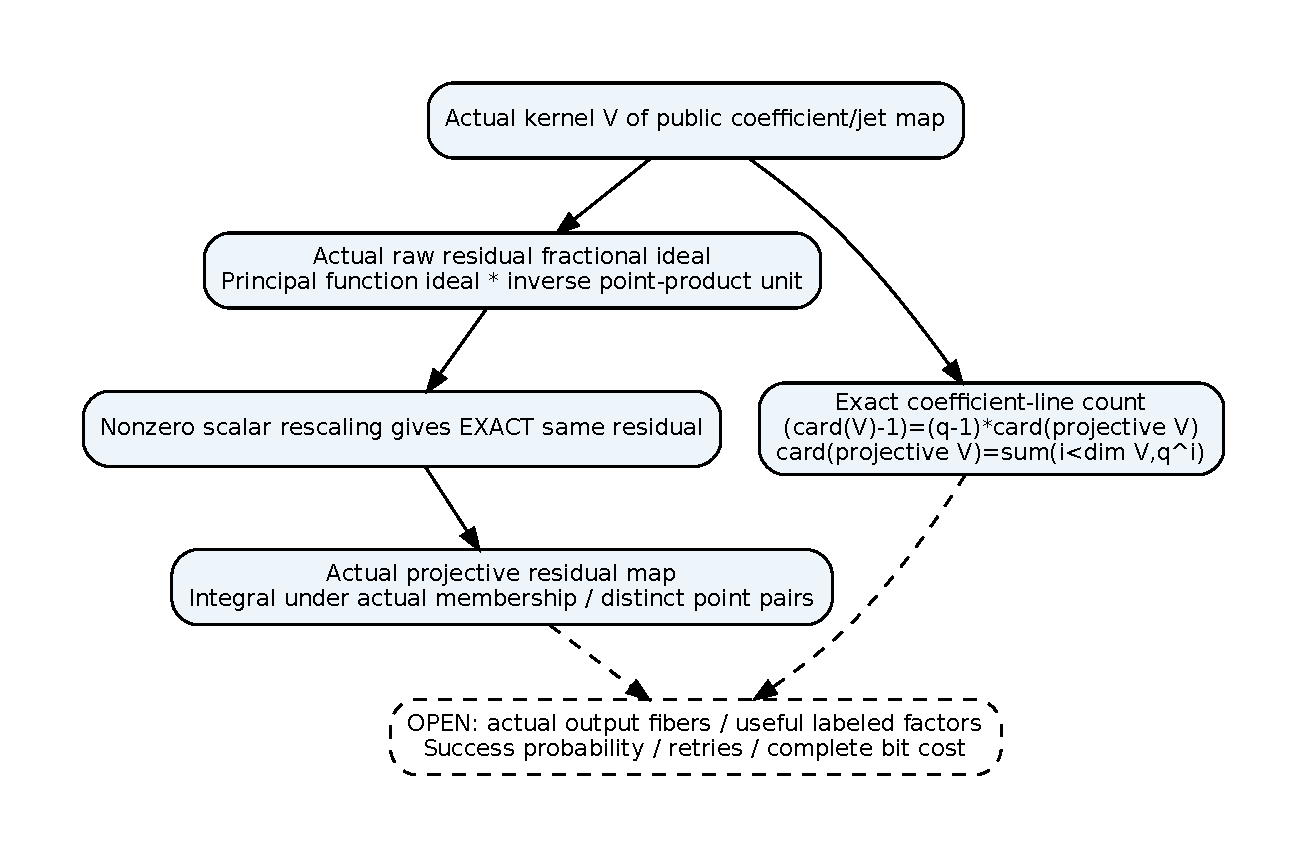
\includegraphics[height=4in,width=.98\linewidth,keepaspectratio]{projective-residual-dependencies-001.pdf}\end{center}
\newpage
\begin{center}{\Large Validation and actual output fibers}\end{center}
\textbf{Lean map.}
Namespace \texttt{OrientationActualProjectiveResidual}, source103/build109/local054:
\begin{center}\begin{tabular}{ll}
\texttt{coefficientIdeal\_rescale}&actual principal ideal unchanged\\
\texttt{rawResidual\_rescale}&actual residual unchanged\\
\texttt{projectiveResidual\_mk}&projective/raw map compatibility\\
\texttt{rawResidual\_integral}&integrality from actual membership\\
\texttt{projectiveResidual\_integral}&integrality on projective inputs\\
\texttt{projective\_count}&exact nonzero-vector count identity\\
\texttt{projective\_count\_finrank}&exact coefficient-line count
\end{tabular}\end{center}
All270 printed statements (seven new) have standard printed foundations;
exit zero, zero warnings and378 exact input bindings checked.
Unlaunched101/pre107 has no build result. Candidate102/build108 exited zero
with two unused-section warnings and was not accepted;103 omitted only the
unused finite-index hypotheses in counting endpoints [pcc:unverified].

\textbf{Next test and scope.}
Determine actual output fibers: equal residuals require actual unit
cancellation and coordinate-ring unit classification before injectivity can
be asserted. No uniform output distribution, rational splitting, known
residual label, success probability or runtime follows yet. Then establish
an actual useful labeled-factor procedure and its class-conditioned
success, retries and complete per-instance bit cost.

\textbf{Sources.}
Actual growing coefficient/residual/unit laws; existing projective
interpolation literature receipt001; public Mathlib ideal singleton-unit
and projectivization lift/cardinality APIs. Standard projective algebra,
no novelty claim; KB unavailable, exact source fallback used. Unsigned
local, outside historical shared Transport53/57 audit/fresh.
Protocol020 and continuation030 retain the next action.
\end{document}
